% using Elseveir template per https://www.elsevier.com/authors/author-schemas/latex-instructions
\documentclass[review]{elsarticle}

\usepackage{amsmath}
\usepackage{lineno,hyperref}
\usepackage{longtable}
\usepackage{booktabs}
\usepackage{hyperref}
\usepackage{siunitx}
\usepackage{tabularx}
\usepackage{threeparttable}  
\usepackage{tikz}

\bibliographystyle{elsarticle-num}
% \journal{Journal of \LaTeX\ Templates}
\modulolinenumbers[5]
\usetikzlibrary{calc,matrix}

% ref: https://tex.stackexchange.com/questions/50747/options-for-appearance-of-links-in-hyperref
\hypersetup{
    hidelinks = true,
}

\begin{document}
\begin{frontmatter}

    \title{
        Conformity and Soft Skills as Determinants of Alternatively Credentialed Non-College Graduate Hireability
    }

    \author[mymainaddress]{John Vandivier}
    \address[mymainaddress]{4400 University Dr, Fairfax, VA 22030}
    \ead{jvandivi@masonlive.gmu.edu}

    \begin{abstract}
        Despite targeting technical skills,
        vocational school graduates earn less than college graduates.
        This paper presents evidence that
        conformity selection and perceived skill gaps explain differences in hireability.
        % Linear models of United States microdata (n=322)
        % reveal a perceived deficit in soft skills for
        % alternatively credentialed non-college graduate (ACNG) labor.
        Microdata from the United States
        reveal a perceived soft skill deficit for
        % Results demonstrate a perceived deficit in soft skills for
        alternatively credentialed non-college graduate (ACNG) labor.
        Conformity is also important,
        but the direction of effect is heterogenous by employer type.
        Conformity and perceived skill gaps explain about one-third of the hireability variance.
        Perceived soft skill gaps explain more hireability variance than widely recognized factors like the industry of occupation.
        Opposite conventional explanation, results suggest that conformity reduces hireability on average.
        Respondents tend to perceive ACNG candidates as an even mix of high and low performers.
        Evidence favors employer risk aversion toward labor productivity as a preferred explanation of low ACNG demand.
        % % Recent college graduates and ACNG job candidates share many of the same perceived skill gaps...
        % % in paper, discuss: sum rulebreaker_ideal rulebreaker_ngwac rulebreaker_recentcollegegraduat rulebreaker_typicalemployeeatmyc
        The conclusion incorporates discussion of public misperception on vocational school costs and suggests activities to reduce unconscious bias.
        % % Results collectively indicate that nontraditional postsecondary education is more valuable than would be expected in the absence of such results.
    \end{abstract}

    \begin{keyword}
        education economics, signaling, hireability, conformity, vocational               %%% not grammatical
        \MSC[2010] I20, I21, J23, J24                                                     %%% not grammatical
    \end{keyword}

\end{frontmatter}

\pagebreak
\linenumbers

\section{Introduction}

% Some optional TODO:
% . talk a bit more about state and industry and see if we can draw a pattern out (STEM industry? high-pop / Democrat states?)
% . `...and employment in the information technology industry yields a positive coefficient`: give beta and sd
% . use table since there are 3 cases of beta and sd (potential TODO: long paper food...2 additional tables; also a summary stats table; perhaps also a diagram)
% . if allowed, another diagram to aid the model section and make the theory clear;

% MB protip: intro outline follows:
% --hook or tension
% --where we are now
% --the importance of your question
% --preview of results

A substantial gap exists between the skills expected by employers and those possessed by college graduates\cite{mcgarry2016examination, malik2017great, abbasi2018analysis, gingras2000there}.
Experts view college alternatives,
including vocational school,
to be useful for technical training,
but the traditional college degree retains a wage premium over vocational education.
Unemployment, underemployment, and other adverse labor outcomes follow a similar pattern\cite{smith_2011}.
This paper seeks to resolve the apparent discrepancy between these outcomes while preserving the mainline economic view that employers pay for perceived job candidate skill.
% or expected marginal revenue product of labor
To explain the apparent discrepancy,
this paper tests the hypothesis that employers expect an offsetting non-technical skill deficit when considering an alternatively credentialed non-college graduate (ACNG).
I find evidence that employers and the general population in the United States expect a low level of soft skills from ACNG job candidates.

Alternative credentials refer to credentials other than the undergraduate degree\cite{brown2017complex}.
The category includes, for example,
industry certifications,
portfolios of work,
digital badges, and other records of unaccredited learning and achievement.
Consumers of alternative education typically intend to leverage alternative credentials toward better employment.
That is, they typically have the same goals as a college student.
Many individuals obtain alternative credentials as a supplement to the college degree.
Supplemental usage is excluded from the analysis in this paper.
This paper focuses on the use of alternative credentials as a substitute for the college degree.
% The level of analysis for this paper dives deeper than the level of credential into skill-level component signal analysis.
This paper provides a comparative analysis between traditional and alternative credentials at the skill level.
Education consumers and learning advisors can use results to inform strategic consumption.
Learning providers can use results as a skill-level diagnostic and product improvement resource.

% Alternative credentials can be obtained quickly and cheaply relative to college.
% Obtaining a college degree signals intelligence, conscientiousness, and conformity,
% but it may not signal technical skill\cite{horton_2020}.
% Alternative credentials signal technical skill.
% As such, they provide an effective supplement to a college degree.

% This paper is concerned with another use case in which a college degree is entirely substituted.
% In that situation, employers may apply a noncollege stigma.
% This is particularly the case for roles which are typically occupied by degree holders.
% Noncollege stigma is a presumption, expectation, or bias toward perception of a skill gap of a certain kind.
% Whether the gap exists in fact is out of the scope of the present paper.

% Technical skill generally implies intelligence.
% Alternative credentials, then, fail to signal two qualities compared to a college degree.
% Alternative credentials fail to signal conscientiousness and conformity.
% Interestingly, some employers may demand some level of nonconformity.
% Employers may also presume a certain lack of soft skill on the part of highly technical applicants.
% % Finally, employers may use alternative credentials as a proxy for other employee characteristics like income, education, race, and gender.

% % a missing link for future research: hireability only correlates with actual hiring decisions it isn't a hiring decision
% Hiring decisions reflect boundedly rational demand for skilled labor.
% a college degree and alternative credentials provide two qualitatively distinct signals of skilled labor.
% The hireability of individuals in possession of these credentials has been studied,
% but the underlying determinants are not clear.
% This paper hypothesizes that perceived skill gaps are important determinants of hireability.
% This paper further hypothesizes that perceived skill gaps are qualitatively different between college graduates and others.
% % In particular, this paper hypothesizes that a noncollege stigma is obtained for candidates without a degree in pursuit of roles typically filled by degree holders.
% % soft skill bias in particular

% three interesting follow-on questions:
%   1. do employers have such a bias
%   2. is such a soft skills gap presumption actually true
%   3. if true, due employers overvalue the soft skills gap
% related paradox: most people won't be in a job for 4-5 years,
% so why do they need to show conscientiousness and conformity towards the 4-5 year bachelor's goal line?
% hard skill stigma: in my experience, people who are highly technical are hard to work with
% soft skill bias: I am favorable bc i think u have soft skills (and maybe this is efficient...enter eq/iq discussion)

% This paper tests the hypothesis that there is a lack of hireability an ACNG (ACNG) is explained by an offsetting perceived lack in non-technical skills.
% In particular, this paper hypothesizes that ACNGs are seen as nonconformist and lacking in soft skills or non-technical skills.
% These deficits explain why an ACNG would not be a preferred source of labor in many cases,
% even if such a candidate does possess superior technical skill.

% technical skill has negative coefficient but magnitude and reliability (p-value/variance) are weaker; overall, less important effect
% hypothesis stems from signaling model.
% This paper proposes skill gaps are perceived in particular among soft skills for alternatively educated individuals.
% one might argue employers are mistaken here; technical work may involve higher, not lower, conscientiousness; ya maybe but out of scope.
% that is, we test social stigma and skill-level / decomposed stigma; an application of the signlaing model.

% Experts view college alternatives including vocational school as useful for technical training, but the traditional college degree retains a wage premium over vocational education.
% This paper hypothesizes that employers pay for skill.
% As a result, lower wages for technically skilled individuals are hypothesized to derive from an offsetting perception of skill deficit elsewhere.
% That is, this paper hypothesizes that employers view an ACNGs (ACNG) as lacking in soft skills.
% This paper hypothesizes that employers expect a skill deficit, although not a technical skill deficit, 
% This expected deficit explains the variance in labor outcomes.

% Sustained rising costs to higher education motivate periodic review of the return to a college degree.
% Despite rising costs, Americans have become more educated than expected over the past decade.
% Trades have contemporaneously seen a labor shortage.

% actually, trade school enrollment is increasing faster than undergraduate enrollment
% https://www.chronicle.com/newsletter/the-edge/2020-01-22
% By 2020, They Said, 2 Out of 3 Jobs Would Need More Than a High-School Diploma. Were They Right?
% overinvestment in college seems to cause a technical labor shortage, but the market is compensating by enrolling more technical folks too
% https://www.theatlantic.com/education/archive/2019/03/choosing-trade-school-over-college/584275/
% undergraduate enrollment has slowed recently and many employers have dropped a college degree requirement
% https://www.npr.org/2019/12/16/787909495/fewer-students-are-going-to-college-heres-why-that-matters
% it is not the case that employers are increasingly demanding a college degree, but it is the case that many do today. Let's examine their reasons.
% peak college?

% As of April 2021, Google Scholar results for the following search terms produce the following counts:
% "human capital theory": 72,300
% "signaling theory": 28,600
% "signalling theory": 16,600
% "screening theory": 4,540
% "control theory": 1,860,000
% "cultural capital theory": 3,830
% "institutional theory": 210,000
% "credentialist theory": 129
% "credentialism": 12,500
% 
% An undergraduate degree is a historically reputable investment.
In a noteworthy literature review, Bills identifies seven sociological or economic theories of the relationship between schooling and job assignment\cite{bills2003credentials}.
A keyword search in April 2021 indicates that human capital theory, institutional theory, and signaling theory are the three theories mentioned by Bills that are most frequently observed\footnote{
    A Google Scholar search for ``institutional theory'' yields about $210,000$ results.
    About two million results are found for control theory, but Bills notes that, ``In its explanatory form, control theory is indistinguishable from human capital theory.''
    In addition, the keyword search results on control theory include disproportionately many results that do not relate to economic analysis.
    The search for `human capital theory' yields about $72,000$ results.
    The sum of `signaling theory' and `signalling theory' is about $45,000$ results.
    The total search result count for the other four theories is less than twenty-five thousand results.
    % The result counts are as follows:
    % "human capital theory": $72,300$,
    % "signaling theory": $28,600$,
    % "signalling theory": $16,600$,
    % "screening theory": $4,540$,
    % "control theory": $1,860,000$,
    % "cultural capital theory": $3,830$,
    % "institutional theory": $210,000$,
    % "credentialist theory": $129$
    % "credentialism": $12,500$,
}.
% The application of institutional theory to education involves `holding constant what they may have learned in school'.
When applied to the economics of education, institutional theory holds that an institution improves individual labor prospects by declaring some individuals to be graduates.
In this application, institutional theory can be included in a signaling model with institutional effects.
In the current study, institutional effects are held constant by using hypothetical questions involving anonymous instititutions.
% line above is sus bc we don't name institutions but we distinguish college grads from ACNGs,
%     and accreditation per se may have some effect that is arguably institutional in a sense
%     but, my conclusions are fine bc i interpret the signal and allow and even suspect that actual skills deviat from signalled skills for grads and acngs

% The signaling model is one of the two standard explanations of the relationship between credentials and labor outcomes\cite{weiss1995human}.
For the purpose of this study, signaling theory provides three advantages over the alternative human capital theory.
First, signaling theory can explain labor outcome variance when human capital unobserved\cite{weiss1995human}.
By extension, signaling theory can also explain labor outcome variance when human capital is held constant.
% First, signaling theory is able to explain labor outcome variance across labor types when skills are totally equal.
% Under a human capital model, in contrast, a variety of labor outcomes would directly imply variance among input labor.
% The present paper expects that skills for the ACNG compared to other labor types are not totally equal, but this must emerge as a result rather than a presumption.

Second, the signaling model empowers a questionnaire research design.
In a standard human capital model of wages, human capital is an input to a production function\cite{hellerstein2007production}.
In a competitive labor market, firms are willing to pay wages equal to the marginal revenue product.
% often MRP is flatly called productivity and defined as human capital
The marginal revenue product for an individual is a function of human capital factors including skills.
Establishing a wide array of such skill measures would be complicated and prone to measurement sensitivities, assumptions, and errors of various kinds.
In this framework, a questionnaire is a second-best design that provides a proxy for the functional measure of skill.

Signaling theory takes the reverse approach.
According to the signaling model, willingness to pay is a function of perceived quality.
The relationship between perceived quality and actual quality is secondary.
In this framework, a questionnaire is an ideal measurement tool.
The value of this research approach is supported by the broad use of questionnaires
to identify willingness to pay within the field of market research\cite{ingenbleek2013best}.

% In this framework, a questionnaire is a direct measure of the functional construct, which is the opinion of the employer.
An additional benefit of using a questionnaire is the ability to ask hypothetical questions.
Hypothetical questions avoid the problem of unobserved heterogeneity
because the analyst has total knowledge over the subject of measurement.

Third, signaling theorists have laid out a testable hypothesis for weak labor outcomes among non-college graduates.
Following this model, scholars claim that the college degree signals intelligence, conscientiousness, and conformity\cite{caplan2018case}.
This paper hypothesizes that, in contrast, alternative credentials signal nonconformity and low conscientiousness.

% Proponents of the signaling model often prefer employer-oriented explanations of college enrollment.
% In this explanation, employers prefer college graduates because the college degree signals intelligence, conscientiousness, and conformity.
% While a technical credential signals intelligence and technical skill, the absence of a degree yields a perceived gap in the mind of the employer.
% There is a perceived comparative lack on the part of the non-college graduate with respect to conscientiousness and conformity.
% This paper tests this hypothesis.

% An agent-based explanation would be that high school graduates are not taught about these alternatives.
% The college degree is popular, has a well-defined return, and is low in risk.
% Particular alternative programs are obscure and often lack a well-defined return.

% Other research indicates that conscientiousness and conformity are not always desirable labor qualities.
% There is some reason to doubt the hypothesis that lower perceived value is attributable to signaling differences in conscientiousness and conformity.
% Research indicates that extreme values for either factor in either direction may be detrimental to productivity.

% TODO: long paper food...uncomment below section as it implies we should be doing marginal analysis. Then do marginal analysis, and K*K skill interactions
% TODO: maybe move to results section when we talk about conscientiousness
% Research indicates a goldilocks level or bliss point for both conscientiousness and conformity is likely to exist.
Employer demand for conscientiousness and conformity follows a bliss point pattern.
Excess individual conscientiousness can disturb team performance\cite{curcseu2019personality}.
Conformity can lead to a lack of innovation and suboptimal organizational practices\cite{symon2006neglected}.
% Psychologists also state that
Conformity selection occurs in part through heuristic cognition or unconscious bias.

% Because a single measure operationalizes each of these effects and their own negation, a fixed sample size is relatively unlikely to identify an important coefficient.
% Because these factors are sometimes demanded and in other cases the inverse is demanded, a factor coefficient may be harder to identify and may only represent the average effect, even if the average effect is hardly predominant in practice.

% The psychological problem is related to but distinct from the pure logical problem that a totally conformed mind is necessarily incapable of innovation.
% Firm innovation requires an underlying capacity for individual innovation.
% Firms must have some capacity for innovation to sustain profit in a growing economy.
% Even if conformity selection is a correct explanation of ACNG aversion, then, it may not be an ideal practice when viewed through the lense of technical or economic efficiency.
% Risk aversion is compatible with a sometimes-concious, sometimes-heuristic decisioning model.

% Innovators, leaders, and high-performers are three kinds of virtuously nonconformant labor.
% Because conformity is sometimes undesirable and sometimes desirable,
% the effect may neutralize itself in an ordinary OLS stastistical analysis.
% The effect may not be identified as important or significant in any particular direction.

Risk aversion is a distinct explanation for conformity selection.
Some employers are not able to evaluate an alternative credential with confidence.
Such an employer views ACNG labor as a gamble with some odds of positive or negative outlier value.
The employer may not prefer to hire such a candidate due to risk aversion,
even if their point estimate for ACNG labor value is higher than their point estimate for a recent college graduate.
If firm size effects are positively associated with ACNG hireability, this will add weight to an explanation based on risk aversion.
% Reasons for this include: 1) failure to deliver can be catastrophic, so low performers may be disproportionately untolerable.
% Revenue consistency, timeline, reputation, quantity produced targeting, large min skill labor cost and marginally small pay increase to achieve adequate production.
% Performance monitoring and turnover costs reinforce this
% zb states I'm assuming constant cost per hire...actually I allow that some portion of large-firm hireability is due to better ability to distinguish low vs high
% other than that effect, the remainder would be attributable to risk aversion.
% yes, the null hypothesis is no difference in cost per hire; but I can also support that which I suspect...turnover costs are proportionally smaller for large firms
% these firms are able to specialize and economize in hiring, plus they are more likely to have high-skill candidates that can better interview and recruitment tech+processes that scales
% TODO: long paper food... consider below articles and flesh out the risk aversion to firm size interaction thing
% note turnover cost calculation is complex but we proxy of just cost to hire. A + B below support cheaper for large firms. (C reinforces B)
%   A) "As stated in a study by the National Association of Colleges and Employers, hiring an employee in a company with 0-500 people costs an average of $7,645."
%   B) "Another study by the Society for Human Resource Management states that the average cost to hire an employee is $4,129, with around 42 days to fill a position."
%   C) "According to Glassdoor, the average company in the United States spends about $4,000 to hire a new employee, taking up to 52 days to fill a position."
% related but doesn't solve the issue: https://builtin.com/recruiting/cost-of-turnover
% https://toggl.com/blog/cost-of-hiring-an-employee
% The highest performing employers, however, will be able to distinguish desirable from undesirable candidates within the unconventional pool.
% Risk aversion varies naturally among firms. <- probably don't write this line in paper as a reviewer can always posit there is a further reason you are missing
% Some employers that are high in risk aversion will provide a net preference to ACNG due to nonconformity preference.

% TODO: long paper food...below section is part of intro or perhaps model...
% \subsection{Process Explanations of Suboptimal Wages}

% Basic price theory holds that an employer should pay wages equal to the marginal revenue product of labor.
% In the real world, measuring candidate productivity at hiring time is costly and imperfect.
% % This produces a technical error which assumes alignment between the goals of the firm and a hiring team.
% A further issue is identified when the hiring team is scrutinized for principal-agent problems.
% The hiring team is composed of individuals with preferences, calculative limitations, and other biases.
% Monitoring and correcting for these problems is expensive,
% so firms will heterogenously realize some aggregation of these individual definiciencies.

% Exacerbating the already necessarily imperfect hiring process are candidate-side problems.
% Firms must hire among a finite, potentially small, number of candidates.
% Risk aversion to time expense and other search costs may lead a firm to approve a suboptimal candidate\cite{simon1976substantive}.
% In some cases, candidate pools may be systematically problematic.
% In law and medicine, for example, extensive education and training are legally required.
% These policies further restrict the candidate pool, inflate expected wages, and systematically alter the content of education in a politically-motivated manner.
% Market forces implement hiring as a lumpy expenditure process to begin with, but certification requirements, wage regulation, and other policies extend the problem.

% The prior discussion highlights many locations of hiring process inefficiency.
% The practical importance of magnitudes and kinds of such effects are described in a legion of related papers.
% A meager sampling of five such effects would include the attractiveness effect and many other issues related to gender bias\cite{quereshi1986physical},
% agentic behavioral stigma\cite{steffens2009feminization},
% and complex biases related to communication style\cite{brouer2017gender, nijs2019effects, sampugnaro1983nonverbal}.
% Sung et al find that impression management meaningfully weakens disability stigma\cite{sung2017disclose}.
% These tactics are transferable in part to noncollege stigma mitigation.
% Finally, there are a wealth of concerns about the effects of social media.
% For one, it presents a channel for the revival of religious discrimination\cite{esposito2018signaling}.

% In the face of so many important inefficiencies, one begins to wonder whether the original theory holds any water at all.
% Papers which identify matching effects, including the present paper,
% serve to limit the proportion of explanation attributable to bias and redeem the elementary price theory story to some extent.
% Prior work demonstrates the important of matching effects in the form of norm compliance\cite{francesco1981gender}.
% Meta-accuracy is a kind of matching measure, and it has been shown to move positively with hireability\cite{renier2018no}.

% \section{Literature Review}
% TODO: long paper food...lit review exists in Announcement effects in the cryptocurrency market
% TODO: long paper food...expand on the signaling model vs the human capital model
% Faster and cheaper alternatives to college exist, but high schools prefer immediate college enrollment over alternative options at a rate of nearly 2:1.
% A New U: Faster + Cheaper Alternatives to College
% Faster and cheaper alternatives to college exist, but the typical student prefers to immediately enroll in college.
% Five student-oriented explanations include an inflated perception of the return to college,
% lack of awareness about alternative programs,
% social pressure to pursue college over alternatives,
% inability to confidently compare returns to alternatives,
% and risk aversion which favors college as a low-risk option despite high cost.


\section{Data and Methodology}
% my model is similar to a Mincer earnings function...but it's not earnings (i could switch income around and maybe get a kind of that)
% https://en.wikipedia.org/w/index.php?title=Mincer_earnings_function&oldid=994739612

A simple model of demand for labor provides context for the hypothesis of interest.
This model is clarified in Equations \ref{eq1} and \ref{eq2}:

\begin{subequations}
    \begin{equation}
        % maybe S is not S_j showing S is a non-person-specific credential
        % but I like S_j because it is *those credentials possessed by j* which can be a unique collection + unique work history, other unique signal, etc...
        S_j = f(H_j)
        \label{eq1}
    \end{equation}
    \begin{equation}
        w_{ij} = E_i(MRP_j) = f_i(S_j)
        % alternatively, D_i(L_j) = E_i(MRP_j) = f(S_j, i)
        \label{eq2}
    \end{equation}
\end{subequations}

Job candidate $j$ generates a signal of productivity $S_j$ from unobserved human capital $H_j$.
Employer $i$, forms an expectation of the marginal revenue product of $j$ on the basis of $f_i(S_j)$, an employer-specific evaluation of $S_j$.
A specific employer is willing to pay a specific job candidate wages of $w_{ij}$.

This study uses ordinary least squares (OLS) regression analysis to estimate the effect of perceived skill gaps on hireability.
An employer is willing to pay more for a relatively hirable individual.
The representation of willingness to pay makes hireability a proxy of demand for labor and $w_{ij}$.
% measure or proxy? proxy bc diff units.
% this is questionable because hireability is technically the willingness to execute a wage integrated over some expected time period (average employee tenure)
% but then, that integrated wage would just be wage multiplied by some constant and we would need to divide by some constant since hireability is a probability
% so, hireability should correlate directly to wage after all
% you also might say hireability is theoretically closer to an estimate of productivity...but who cares it's once again equal
% and we want to frame the overall model as a simple labor demand model.
%
% Equally, a respondent is making an expected productivity statement when scoring hireability
% This study presumes that employers are willing to pay less for an ACNG.
% This study also presumes that ACNG labor has better technical skill.
This paper hypothesizes that employers preferentially value soft skills in the course of $f_i(S_j)$
to explain the reduced willingness to pay for ACNG labor relative to college graduate labor.
If employers do bias toward soft skills in job candidate evaluation,
one or more soft skill gap factors should yield a negative coefficient
in a regression on hireability.

This paper leverages an original set of online questionnaire responses ($n = 322$).
Responses are cross-sectional data obtained in early February of 2021.
Respondents are United States citizens at or over the age of eighteen.
Qualified respondents participated in the survey through the Amazon Mechanical Turk platform.

The survey includes 65 questions in two sections\footnote{See Appendix A for a full copy of the survey.}.
The first section captures respondent characteristics, and the second section captures a skill-level evaluation of various hypothetical job candidates.
Grouping these variables into three groups simplifies discussion.
There is the dependent variable of interest, independent variables of interest, and categorical controls.

In this study, the categorical variables and the control variables are the same set.
The independent and dependent variables of interest are Likert-type responses on a 10-point scale
% Employer responses did not significantly differ from the general population,
% so results generally hold for both employers and the United States population.
\footnote{
    It is an accepted practice to treat Likert-type responses as either categorical or continuous for regression analysis.
    % This paper treats such variables as continuous, which is consistent with the theoretical structure of the demand curve and the other variables of analysis.
    % it's also consistent with normalized reporting of real skill measurement; even percentiles themselves are continuous entities.
    % ie, I could do marginal analysis; and i did a little but i'm not talking about it lol.
    Jaccard and Wan provide support for continuous analysis of Likert-type data.
    They note that severe departures from the assumptions on cardinality ``do not seem to affect Type I and Type II errors dramatically,''
    particularly when the Likert scale is five or more points\cite{jaccard1996lisrel}.
    This paper uses a 10-point scale and treats these data as continuous.
    % A 10-point scale is equivalent to a continuous response from 1 to 10 with rounding.
    %
    % In the current data set, continuous treatment provides a consistent and conservative fit of the data with high confidence.
    % Categorical decomposition yields higher fit with less significance in each category of Likert response.
    % This indicates categorical decomposition may represent a case of overfit and is therefore an additional reason not to prefer that analytical approach.
    %
    % % TODO: long paper food...add marginal fx and u get a third reason Likert as continuous is gtg
    % Finally, treating Likert-type responses as continuous is structurally defensible in this particular study.
    % The notion that Likert-type responses are purely ordinal would make the notion of marginal effect absurd and incalculable,
    % but willingness to pay for labor, conscientiousness, and other factors used in this study are known to exhibit marginal effects in the literature. % TODO: I could cite but it's pretty obv
    % See the results section where a marginal effect from conscientiousness is identified and interpreted in a meaningful way.
    %
    % TODO: but probably not...I could also cite a paper where an economist uses Likert questionnaire data as cardinal
    % i would be happy to use a categorical-like treatment if not for this, and the latter might even have better fit but it could be overfit.
    % finally, an alternative approach would be to treat likert responses as categorical, but the continuous treatment has less fit and more structural justification
    % categorical treatment is a relative overfit
    % likert-type units can be considered direct psychological measures or economic proxies.
    % The likert-type response curve can be thought of as a function of actual skill;
    % b. decent paper on ordinal independent variables: https://www3.nd.edu/~rwilliam/stats3/OrdinalIndependent.pdf
    % c. more on this: https://www.researchgate.net/post/Is_a_Likert-type_scale_ordinal_or_interval_data
}.
Higher Likert-type values indicate greater agreement with the associated statement.
Categorical controls include state of residence,
the industry of occupation,
employer status,
firm size,
and a measure called duration.

% https://stats.stackexchange.com/questions/539/does-it-ever-make-sense-to-treat-categorical-data-as-continuous
% I treat duration as continuous even though it is categorical, but the likert-type defense applies statistically.
Duration measures the length of time the respondent believes it takes to obtain an alternative credential.
Employer status describes whether an individual makes hiring and firing decisions in the course of their employment.
The variable takes one of three values: yes, no, or unemployed.
Employer effects refer to the case where an individual states that they do make hiring and firing decisions.
State of residence refers to a state within the United States or the District of Columbia.
% While it was permitted, only one actual response identified the District of Columbia as a residence.

The dependent variable of interest is called hireability.
Hireability measures agreement that, ``For many professions, alternative credentials can qualify a person for an entry-level position.''
The dependent variables of interest include perceived skill gaps and rulebreaker effects.

% The unit of factor coefficients for nonconformists and skill gaps is hireability per Likert-type unit, where hireability is also a Likert-type unit.
% Rulebreaker effects refer to a collection of three factors that describe the way employers think about nonconformists, or "People who are willing to break formal or informal rules and norms."
Rulebreaker effects refer to a collection of three factors that measure respondent agreement with statements about nonconformists, or ``People who are willing to break formal or informal rules and norms.''
% The three rulebreaker questions measure respondent agreement with statements 
The first statement indicates that nonconformists present a risk to a company's reputation, productivity, or value.
This statement received the least agreement and greatest response variance
among three qualitatively different descriptions of nonconformists ($\mu = 6.29, \sigma = 2.51$).

The second statement indicates that nonconformists are held back by rules,
and ``could just as easily be high performers as low performers.''
% The second statement indicates that people break rules which hold them back, and that nonconformists "could just as easily be high performers as low performers."
% MAYBE TODO: standard error instead of or in addition to standard deviation. maybe make a table since there are at least three cases of similar report.
This statement received the most agreement and least variance among rulebreaker statements ($\mu = 6.93, \sigma = 2.10$).
The agreement with this statement provides evidence against the thesis that employers value conformity for its own sake.
In turn, this adds weight to the theory that employers value conformity as a risk aversion tactic while knowing that nonconformity signals positive outlier potential.
The third rulebreaker effect states that rulebreakers are creative, innovative, and likely to benefit company culture ($\mu = 6.71, \sigma = 2.18$).
% managers are wary of ACNG, having high correlation with "Rule Breakers Risky"
% reg _ismanager1 rulebreakersnormsmightbedoingsob rulebreakersnormsprobablyhaveaha rulebreakersnormstendtobegiftedi

% % MAYBE TODO: sentence below can be shortened and we can introduce likert-type unit as distinct from likert-type response since it's a computed value
% Perceived skill gaps are computed from perceived skill questions in the second section of the survey.
% % Respondents do not directly report perceived skill gaps.
% % Instead, responses indicate perceived skill level for particular skill and a particular type of job candidate.
% % 13 skills are analyzed and 4 job candidate types are surveyed, for a total of 52 questions in the second section on perceived skill.
% % MAYBE TODO: citation to "make response anchoring appropriate"
% % Each section begins with a contextual message to normalize response anchoring.
% % Questions are provided in nonrandom order for the same reason.
% % Data from the second section is used to calculate perceived skill gaps.
% For each of 13 skills, the respondent is asked to imagine four types of job candidate.
% One type of candidate is an ideal candidate.
% Raw perceived ACNG skill gaps are calculated by differencing the perceived skill of an ideal candidate with the perceived skill of an ACNG.
% % technically, the actual skill of an ideal candidate equals the perceived skill so the adjective is extraneous; but let's be consistent and not confuse reader.

Rulebreaker effects and perceived skill gaps are structurally linked.
One of the skills that respondents evaluate is nonconformity, or ``willingness to break formal or informal rules and norms.''
Interpreting rulebreaker effects jointly with the conformity gap effect
% Joint interpretation of nonconformity and rulebreaker effects
enables better explanatory power and diagnostic utility.
% Explanatory power is improved because conformity has potential benefits and costs.
% Aggregating these effects under a single variable creates noise.
% Explanatory power is improved because employers can express that they value conformity either per se or as a proxy for some other qualities.
% Diagnostic utility is improved because alternative learning providers may be able to accomodate whatever non-per-se qualities employers value.

Perceived skill questions in the second section of the survey allow for two ways to calculate perceived skill gaps.
Perceived skill gaps are measured separately with and without overqualification effects.
Overqualification effects are important in external research\cite{green2007there, raybould2005over}, but skill gap analysis that ignores these effects is also routine\cite{blake_2018}.
% MAYBE TODO: cite more than 1 person who ignores overqualification
% MAYBE TODO: just have one dependent variable and don't mention the other. it's something i did at analysis time, but may be confusing in the paper.
%       alternatively, keep 'em both and call the second a robustness test...that is what i use it for anyway

Perceived skill is a Likert-type response reporting agreement stating that a particular candidate has a particular skill.
For each of 13 skills, the respondent imagines and reports skill levels for the ideal candidate,
the average actual employee,
the average recent college graduate,
and the average ACNG.
As a result, 52 of the 65 questions in the survey are questions on perceived skill about kind of candidate.

The raw skill gap for a candidate is the difference between the perceived skill for that candidate and the ideal candidate.
The perceived skill gap with overqualification effects equals the raw perceived skill gap.
The perceived skill gap without overqualification is zero if the raw skill gap is negative,
and otherwise, it is equal to the raw skill gap.

The concept of skill is intentionally treated loosely in this analysis.
The thirteen factors treated as skills include
attractiveness,
verbal, written, and body language communication skills,
conscientiousness,
customer service skill,
emotional intelligence (EQ),
expected salary,
teamwork,
technical skill,
willingness to break formal or informal rules (nonconformity),
willingness to work odd hours,
and willingness to commute.
% TODO: discuss attractiveness halo effect

Results focus on ACNG skill gap coefficients
and also comparative skill gaps between ACNG labor and recent college graduates.
Perceived ACNG skill gaps are also called absolute skill gaps.
Subtracting the perceived recent college graduate skill gap from the absolute skill gap yields the comparative skill gap.
% In this study, overqualification effects ended up reducing explanatory power, so they are largely ignored.

Models of these variables will support the hypothesis if soft skills are more important than technical skill gaps.
Significant rulebreaker effects would provide evidence that conformity is valued differently for different types of employers.
A positive relationship between firm size and hireability would support an explanation from risk aversion.
% MAYBE TODO: I also expect signs to be generally negative and soft skills should be statistically significantly less for ACNG compared to recent college graduate

% simple match effect: those that prefer technical talent will tend to support alternative credentials.
% complex match effect: a match profile will have significantly and importantly more explanatory power compared to but consistent with a simple match effect.

% quality question meta: 1 to 10: disagree to agree
% ---
% An ideal candidate would have this quality...
% A typical employee would have this quality...
% A college graduate would have this quality...
% A credentialed or certified non-college graduate would have this quality...
% [later] Someone who is self-taught (without a credential or portfolio) would have this quality...
% [later] A typical junior-level high school student would have this quality...

% some notes, mainly out of scope
% ---
% hiring error awareness increases in a few ways
%  1. [passive search] participant observation. As an interviewer, interviewee, hiring manager, or other professional involved in the process, I simply notice a problem
%  2. [passive search] passive company and individual level search into HR best practices; an industry newsletter says hey Griggs v Duke happened so don't use IQ tests anymore.
%  3. [passive search]: audit compliance (legal+required, or optional audits from firms that certify quality, for example)
%       example: Supreme Court case Griggs v Duke had an industry-wide effect thru this means
%  4. [active search] intrapraneurship / policy change championing begins with an individual saying hey let's investigate this thing. what would motivate such individual? (maybe due to 1 or 2).
%
% my prior work has shown that we can predict (r2 0.5 - 0.7 and ar2 0.3 - 0.6) alternative education hireability from employer factors alone - without concern to matching

\section{Results}

% Hireability in this study is called favorability in the COVID study.
% Here, I want to highlight the theoretical connection to willingness to pay.
% In the other study, I wanted to highlight the psychometric connection to familiarity bias and so forth
The median hireability response was eight out of ten.
The mean response is about 7.42.
% Of 322 responses, 10 responses indicate a hireability of less than four out of ten.
% Partial responses were submitted in 21 cases, but partial responses did not impact factors in models of interest.
Absolute skill gaps and comparative skills gaps are both important explanations of hireability.
Soft skills explain hireability better than technical skill does in both absolute and comparative terms.
Technical skill is not a contributing factor in any model of interest.
Of the thirteen skills investigated, seven skills contribute to the preferred model.

% TODO: skill gap ols, gap of gaps ols

% TODO: final ols

% TODO: consider RLM, GLM, and control variables.

% TODO: maybe Compare directly to bootcamp results from Indeed: https://www.indeed.com/lead/what-employers-think-about-coding-bootcamp

% TODO: in preferred model, discuss Duration forced in, don't worry bout multicollinearity bc N/A dropped; rulebreaker gaps forced in

% \subsection{A Model of Absolute Skill Gaps}

Table \ref{tab:table_new_ols} reports five interesting multiple regressions.
Models 1 through 4 maximize adjusted r-squared for a given set of factors.
Factors in these models are not constrained using a p-value threshold.
Model 4 is the preferred model, and factors in this model have a p-value less than $0.28$.
Model 5 is a special case designed to answer an analytical question.

Models 1 and 2 maximizes adjusted r-squared using absolute skill gaps.
Model 1 includes overqualification effects, and Model 2 excludes these effects.
This model is useful to demonstrate which skills are important determinants of ACNG hireability.
The key result from these two models is that measuring skill gaps without overqualification is preferred.

Models 3 through 5 also exclude overqualification effects.
Model 3 maximizes adjusted r-squared using comparative skill gaps.
This model explains hireability by comparing ACNG labor to recent college graduates by skill.
Model 4 synthesizes comparative and absolute skill gaps.

% derived from analysis-5-regs-table.do
{
\def\sym#1{\ifmmode^{#1}\else\(^{#1}\)\fi}
\begin{tabular}{l*{5}{c}}
\toprule
                         &\multicolumn{1}{c}{1}&\multicolumn{1}{c}{2}&\multicolumn{1}{c}{3}&\multicolumn{1}{c}{4}&\multicolumn{1}{c}{Model 5}\\
\midrule
Is Employed Non-Manager  &      -0.336         &      -0.383\sym{*}  &      -0.497\sym{**} &      -0.471\sym{**} &      -0.451\sym{**} \\
\addlinespace
Is STEM Worker           &      -0.491\sym{**} &      -0.529\sym{**} &      -0.525\sym{**} &      -0.557\sym{**} &      -0.564\sym{**} \\
\addlinespace
Employees 51-200         &      -0.475\sym{*}  &      -0.480\sym{**} &      -0.364         &      -0.459\sym{*}  &      -0.457\sym{*}  \\
\addlinespace
Industry Credentials Legally Required&       0.706\sym{*}  &       0.722\sym{**} &       0.374         &       0.378         &       0.375         \\
\addlinespace
Industry Credentials Normal&       0.932\sym{**} &       0.926\sym{**} &       0.487\sym{*}  &       0.436\sym{*}  &       0.448\sym{*}  \\
\addlinespace
Industry Credentials Sometimes Used&       0.467         &       0.475         &                     &                     &                     \\
\addlinespace
Industry Credentials Unknown&       0.641\sym{*}  &       0.684\sym{**} &                     &                     &                     \\
\addlinespace
Industry, Agriculture    &       1.368         &       1.619\sym{*}  &                     &                     &                     \\
\addlinespace
Industry, Energy         &      -1.277\sym{*}  &      -1.190\sym{*}  &      -1.200\sym{*}  &      -1.442\sym{**} &      -1.448\sym{**} \\
\addlinespace
Industry, Finance, Investment, or Accounting&      -0.811\sym{***}&      -0.783\sym{***}&      -0.712\sym{***}&      -0.715\sym{***}&      -0.717\sym{***}\\
\addlinespace
Industry, Information Technology&       0.335         &       0.264         &       0.438\sym{*}  &       0.306         &       0.337         \\
\addlinespace
Industry, Law            &      -1.813\sym{***}&      -1.670\sym{**} &      -1.935\sym{***}&      -1.876\sym{***}&      -1.857\sym{***}\\
\addlinespace
Industry, Transportation &       1.512\sym{*}  &       1.643\sym{**} &       1.216         &       1.403\sym{*}  &       1.350\sym{*}  \\
\addlinespace
State, Arizona           &      -1.157\sym{**} &      -1.048\sym{**} &      -0.755         &      -0.823\sym{*}  &      -0.790         \\
\addlinespace
State, Arkansas          &      -2.690\sym{***}&      -2.817\sym{***}&      -2.489\sym{***}&      -2.664\sym{***}&      -2.770\sym{***}\\
\addlinespace
State, California        &      -0.575\sym{*}  &      -0.570\sym{**} &      -0.488\sym{*}  &      -0.435         &      -0.446         \\
\addlinespace
State, Colorado          &      -1.446\sym{**} &      -1.423\sym{**} &      -1.463\sym{**} &      -1.521\sym{***}&      -1.508\sym{***}\\
\addlinespace
State, Connecticut       &      -1.401         &      -1.550         &                     &                     &                     \\
\addlinespace
State, Florida           &      -0.444         &      -0.454         &                     &                     &                     \\
\addlinespace
State, Hawaii            &      -3.232\sym{***}&      -3.271\sym{***}&      -2.884\sym{***}&      -2.869\sym{***}&      -2.812\sym{***}\\
\addlinespace
State, Illinois          &      -0.637         &      -0.699\sym{*}  &      -0.596         &      -0.675\sym{*}  &      -0.698\sym{*}  \\
\addlinespace
State, Kansas            &      -3.283\sym{**} &      -3.486\sym{**} &      -2.923\sym{*}  &      -3.116\sym{**} &      -3.101\sym{*}  \\
\addlinespace
State, Kentucky          &      -3.143\sym{***}&      -3.167\sym{***}&      -2.583\sym{***}&      -2.729\sym{***}&      -2.679\sym{***}\\
\addlinespace
State, Louisiana         &      -1.455\sym{*}  &      -1.255\sym{*}  &      -0.915         &      -0.941         &      -0.898         \\
\addlinespace
State, Maryland          &      -0.596         &      -0.642         &                     &                     &                     \\
\addlinespace
State, Nebraska          &      -2.037\sym{*}  &      -2.167\sym{*}  &      -1.391         &      -1.655         &      -1.596         \\
\addlinespace
State, Nevada            &      -1.406         &      -1.470         &      -1.465         &      -1.434         &      -1.409         \\
\addlinespace
State, New Jersey        &      -1.145         &      -1.139         &      -0.976         &      -0.936         &      -0.963         \\
\addlinespace
State, New York          &      -0.692\sym{**} &      -0.640\sym{*}  &      -0.617\sym{*}  &      -0.595\sym{*}  &      -0.590\sym{*}  \\
\addlinespace
State, Ohio              &      -3.943\sym{***}&      -4.024\sym{***}&      -4.051\sym{***}&      -3.808\sym{***}&      -3.761\sym{***}\\
\addlinespace
State, Pennsylvania      &      -0.752         &      -0.687         &      -0.608         &      -0.534         &      -0.539         \\
\addlinespace
State, South Carolina    &      -1.183         &      -1.243         &      -1.361         &      -1.310         &      -1.347         \\
\addlinespace
State, Tennessee         &      -1.878\sym{**} &      -1.909\sym{**} &      -1.545\sym{*}  &      -1.843\sym{**} &      -1.799\sym{**} \\
\addlinespace
State, Texas             &      -0.906\sym{**} &      -0.851\sym{**} &      -0.797\sym{**} &      -0.790\sym{**} &      -0.789\sym{**} \\
\addlinespace
State, Washington        &      -0.817         &      -0.863\sym{*}  &      -0.880\sym{*}  &      -0.996\sym{**} &      -1.003\sym{**} \\
\addlinespace
Duration                 &       0.666\sym{**} &       0.634\sym{**} &       0.811\sym{***}&       0.744\sym{**} &       0.719\sym{**} \\
\addlinespace
cduration2               &     -0.0884\sym{**} &     -0.0857\sym{**} &      -0.113\sym{***}&      -0.103\sym{**} &     -0.1000\sym{**} \\
\addlinespace
WOQ, Gap, Attractiveness &      -0.161\sym{***}&                     &                     &                     &                     \\
\addlinespace
WOQ, Gap, Body Language-IT&       0.100         &                     &                     &                     &                     \\
\addlinespace
WOQ, Gap, Conscientiousness&     -0.0657         &                     &                     &                     &                     \\
\addlinespace
WOQ, Gap, EQ             &     -0.0966         &                     &                     &                     &                     \\
\addlinespace
Rule Breakers Risky      &      0.0732\sym{*}  &      0.0715\sym{*}  &      0.0880\sym{**} &      0.0747\sym{*}  &      0.0762\sym{*}  \\
\addlinespace
Rule Breakers Rockstars  &       0.133\sym{**} &       0.128\sym{**} &       0.147\sym{**} &       0.141\sym{**} &       0.140\sym{**} \\
\addlinespace
Rule Breakers Culture Add&      0.0905         &      0.0974\sym{*}  &       0.115\sym{**} &       0.112\sym{**} &       0.110\sym{**} \\
\addlinespace
Gap, Attractiveness      &                     &      -0.367\sym{***}&                     &      -0.350\sym{***}&      -0.358\sym{***}\\
\addlinespace
Gap, Body Language-IT    &                     &       0.132         &                     &       0.106         &      0.0874         \\
\addlinespace
Gap, Conscientiousness   &                     &     -0.0845         &                     &      -0.132\sym{**} &      -0.134\sym{**} \\
\addlinespace
Gap, EQ                  &                     &     -0.0952         &                     &                     &                     \\
\addlinespace
Comparative, Attractiveness&                    &                     &      -0.185\sym{*}  &                     &                     \\
\addlinespace
Comparative, Conscientiousness&                     &                     &      -0.140         &                     &                     \\
\addlinespace
Comparative, Customer Service&                     &                     &       0.138         &       0.142\sym{*}  &       0.145\sym{*}  \\
\addlinespace
Comparative, EQ          &                     &                     &     -0.0955         &                     &                     \\
\addlinespace
Comparative, Willing to Work Odd Hours&                     &                     &      -0.177\sym{*}  &      -0.255\sym{***}&      -0.260\sym{***}\\
\addlinespace
Comparative, Teamwork    &                     &                     &      -0.196\sym{*}  &      -0.242\sym{**} &      -0.251\sym{**} \\
\addlinespace
Comparative, Written Communication&                     &                     &       0.128         &      0.0920         &      0.0934         \\
\addlinespace
Comparative, Rulebreaker &                     &                     &                     &                     &      0.0182         \\
\addlinespace
Gap, Rule Breaker        &                     &                     &                     &                     &      0.0574         \\
\addlinespace
Constant                 &       5.036\sym{***}&       5.356\sym{***}&       4.755\sym{***}&       5.327\sym{***}&       5.343\sym{***}\\
\midrule
R-sqr                    &      0.3253         &      0.3539         &      0.3310         &      0.3706         &      0.3721         \\
p(F)                     &      0.0000         &      0.0000         &      0.0000         &      0.0000         &      0.0000         \\
N                        &         322         &         322         &         322         &         322         &         322         \\
\bottomrule
\multicolumn{6}{l}{\footnotesize Standard errors in parentheses}\\
\multicolumn{6}{l}{\footnotesize \sym{*} \(p<0.10\), \sym{**} \(p<0.05\), \sym{***} \(p<.01\)}\\
\end{tabular}
}


Rulebreaker effects are significant in all models.
Nonconformity is insignificant in a multiple regression that includes rulebreaker effects.
The insignificance of nonconformity is intuitive because these factors essentially describe the same thing.
Rulebreaker effects describe the way a respondent qualitatively views conformity.
Excluding overqualification, a conformity skill gap indicates that a respondent views ACNG labor as less conformist than ideal.
The way a respondent views conformity substantially implies their ideal level of conformity and how deviations from that ideal will impact willingness to hire.
This implication is substantial but imperfect.
Because the implication is substantial, a conformity skill gap does not improve adjusted r-squared.
Because the implication is imperfect, there is an opportunity to force the conformity skill gap into the model.
While the p-value will be unacceptably high, it is still analytically interesting to obtain the direction of the conformity skill gap effect.
This is what Model 5 does.

Model 5 takes Model 4 and adds additional factors for employer size,
the absolute skill gap for conformity,
and the comparative gap for conformity.
These factors are insignificant, so the coefficient does not provide a confident estimate of the magnitude of the effect.
The signs of the effects do add marginally to the cumulative evidence for conclusions.
Rulebreaker effects are robustly positive and significant in all models.
Positive rulebreaker effects indicate that nonconformity is positive on hireability.
The positive coefficients on nonconformity skill in Model 5 reinforce this result.

Employer size is a categorical variable, so regression technically treats this variable as a series of dummies.
One employer size dummy contributes to Model 4, and it has a negative coefficient.
The negative coefficient might appear to be evidence against the claim that large employers
are more favorable to ACNG labor.
However, the dummy in Model 4 represents an employer size that is less than average.
The implication is that the model constant contains a positive effect for larger employers.
Model 5 reinforces the subtle implication.
Model 5 contains positive coefficients for most firm sizes, including firms at or above the median size.

Figure \ref{fig:firm_size} adds to the evidence that large firms favor alternative credentials.
Firm size is a categorical variable with nine possible responses.
Figure \ref{fig:firm_size} plots a numeric transform of the variable along the horizontal axis.
The vertical axis represents the frequency of response for a given value.
Responses from one through eight represent increasing intervals of firm size.
The negative coefficient on employer size in Model 4 corresponds to a response of three in the horizontal axis.
A response of nine indicates that the question is not applicable because the respondent is not employed.
The ninth response is dropped from Model 5 to prevent multicollinearity.
There is no loss of analytical power in Model 5 because the dropped dummy does not represent firms of any size.
This figure further illustrates that the negative coefficient pertains to small firms.
The high willingness to hire on the part of large employers adds to the explanation of low ACNG labor demand from risk aversion.

\begin{figure}[h!]
    \centering
    \caption{Distribution of Firm Size}
    \begin{tikzpicture}[element/.style={minimum width=1.75cm, minimum height=0.85cm}]
        \node (n1) {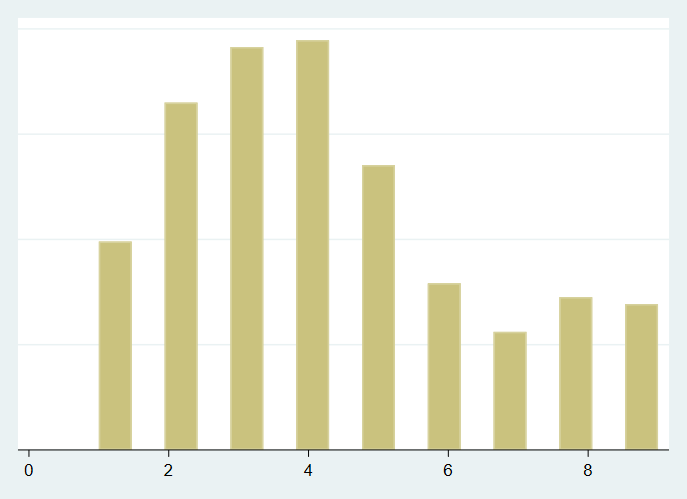
\includegraphics[width=0.8\textwidth]{./figures-and-tables/firm-size-hist.png}};
        \node (n2) [above=0.25cm] at ($(n1)!0.5!(n1) - (5.75, 0)$) {\textbf{Density}};
        \node (n3) [above=0.25cm] at ($(n1)!0.5!(n1) - (0, 4.5)$) {\textbf{Discretized Firm Size}};
    \end{tikzpicture}
    \label{fig:firm_size}
\end{figure}

Models are specified using ordinary least squares (OLS).
A robust linear model (RLM) and a generalized linear model (GLM) verify OLS results.
RLM and GLM specification alters factor significance but does not alter the coefficient value.
RLM and GLM models account for abnormal factor distribution.
In the OLS specification of Model 4, the preferred model, p-values did not exceed 0.28.
In RLM specification, p-values did not exceed 0.41.
In GLM specification, p-values did not exceed 0.38.
Overall, OLS seems slightly overfit, and RLM seems slightly underfit compared to GLM.
This analysis is mainly concerned with the direction of factor effects
rather than a precise estimate of coefficient magnitudes.
The important result from robustness testing is that coefficients did not change,
and the direction for each factor is plausible ($p < 0.5 < p'$).

Model 4 identifies seven skill gaps as important explanatory factors.
Four important skill gaps are comparative, and three are absolute gaps for ACNG candidates.
Figure \ref{fig:important_gaps} illustrates the distribution for each important skill gap.
Reflecting on this figure helps inform a diagnostic analysis for use by alternative learning providers.
ACNG candidates can also supplement their learning to address these gaps.
A simple remedy does not seem to apply for attractiveness and willingness to work odd hours.
Conscientiousness is difficult to train, but analysis suggests perception management as a remedy.
% corr cduration1 aetiwo_conscientiousness => 0.21
Perceived conscientiousness has a slight correlation duration (Pearson's $r = 0.21$).
Spending additional time to obtain a credential is a way to improve perceived conscientiousness.
ACNG supplementation of a credential with additional self-study time may also improve perceived conscientiousness.
% External research indicates that psychological therapy and other interventions can boost conscientiousness in some cases\cite{kilduff_tasselli_landis_2018}.

The important body language communication gap is an interaction with the information technology industry variable.
The interaction indicates a reduced penalty for lack of body language communication skills
in the information technology industry.
A reduced penalty for soft skill deficit helps explain the particular flourishing of
alternative credentials in the information technology industry.
The reduced penalty in this particular industry might be related to its relative lack of regulation.
Another hypothetical explanation is that the reduced penalty is related to cultural norms in the industry.
Suppose that there is a diminished technical need for social skills in programming.
In that case, introverts obtain a comparative advantage in this field.
Further study that includes personality data is encouraged to test this hypothesis.
The interacted body language skill gap and the customer service skill gap
are interesting for niche learning providers.

\begin{figure}[h!]
    \centering
    \caption{Distribution of Important Gaps}
    \begin{tikzpicture}[element/.style={minimum width=1.75cm, minimum height=0.85cm}]
        \node (n1) {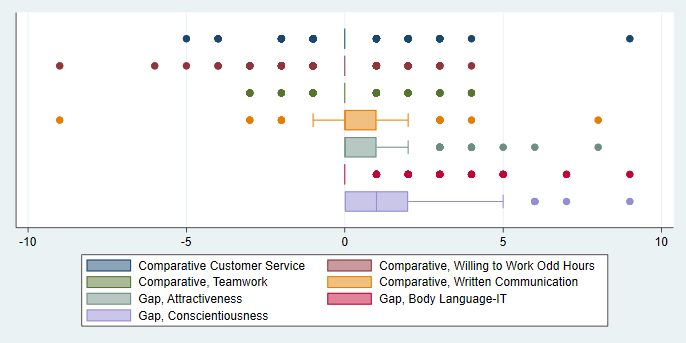
\includegraphics[width=1\textwidth]{./figures-and-tables/skill-bars.png}};
    \end{tikzpicture}
    \label{fig:important_gaps}
\end{figure}

The gaps in teamwork and written communication skill seem to be the best candidates for
feasible remedy with broad learning provider applicability.
Written communication skill is uniquely amenable to online learning.
Written communication skill is also unique in the response distribution.
The written communication skill gap is a comparative gap where the interquartile range favors ACNG labor.
This indicates the perception that ACNG providers are generally capable of providing this skill.
The distribution reflects positive and negative outliers.
Positive outliers indicate that the typical provider can improve by emulating market leaders.
Negative outliers indicate that some learning providers are particularly poor at training this skill.
If learning providers are generally effective in training this skill,
improvement for ineffective providers is likely to be feasible.

% TODO: maybe cite some literature on digital social learning or project-based learning
Alternative learning providers can use project-based learning and social learning
techniques to facilitate teamwork skill development.
These are not the most common pedagogies, but they are an established and effective pattern.
An online environment can implement courses with project-based learning and social learning.
The distribution of responses indicates that improving teamwork skill has neither the maximum
penalty nor the maximum return potential compared to improving written communication.
Model results preclude decisive prioritization of written communication skills.
Model 4 indicates that the effect of teamwork skill on hireability is more reliable
and larger in magnitude compared to the coefficient on written communication skill.
Targeting both of these two skills is feasible and beneficial to educational quality.
% where educational quality is defined as plausible impact to labor outcomes

The preferred model explains about one-third of hireability variance,
but how much of the explanatory power is attributable to skill gaps?
Table \ref{tab:explantory_power} provides evidence on the importance of perceived skill gaps and rulebreaker effects
relative to other factor groups.
Model 4 is composed of factor groups.
Table \ref{tab:explantory_power} summarizes results for simple regressions of each factor group on hireability.
Industry and state effects are factor groups regarded in external literature as important for models in the labor market.

\begin{table}
    \caption{Factor Group Explanatory Power in a Simple Regression with Hireability as Dependent Variable}
    \resizebox{\columnwidth}{!}{
        {
\def\sym#1{\ifmmode^{#1}\else\(^{#1}\)\fi}
% \begin{center}
{
    \fontsize{8pt}{7pt}\selectfont
    % \begin{small}
    \tabcolsep=3pt
    \begin{tabular}{l*{4}{c}}
        \toprule
        \multicolumn{1}{c}{Effect Group} & \multicolumn{1}{c}{Adj R-Sqr} & \multicolumn{1}{c}{R-Sqr} & \multicolumn{1}{c}{Max p-value} \\
        \midrule
        Absolute Gap                     & 0.0615                        & 0.0703                    & 0.097                           \\
        \addlinespace
        Comparative Gap                  & 0.0176                        & 0.0298                    & 0.687                           \\
        % \addlinespace
        % Rulebreaker                           & 0.1432                        & 0.1554                    & 0.053                           \\
        \addlinespace
        Industry                         & 0.0303                        & 0.0454                    & 0.958                           \\
        \addlinespace
        \addlinespace
        Other Factors                    & 0.0072                        & 0.0288                    & 0.537                           \\
        \addlinespace
        Rulebreaker                      & 0.0783                        & 0.0869                    & 0.127                           \\
        \addlinespace
        State                            & 0.0469                        & 0.1033                    & 0.772                           \\
        % \addlinespace
        % State, Semi-Robust                    & 0.0034                        & 0.0648                    & 0.831                           \\
        \bottomrule
    \end{tabular}
    % \end{center}
}
}

% TODO: maybe a count of k factors in group
% TODO: maybe distinguish strong and weak effects for industry, state, and gaps
% TODO: maybe other controls / other factors section doesn't matter
% TODO: maybe combine skill gaps

    }
    \label{tab:explantory_power}
\end{table}

Table \ref{tab:explantory_power} shows that perceived skill gaps and rulebreaker effects explain more
variance in hireability compared to the state, industry, and other effects.
Industry and state effects are also less stable.
A simple model of industry effects on hireability results in some industry effects approaching a p-value of 1.
In contrast, the least significant absolute skill gaps are statistically significant in a simple regression ($p < 0.1$).
% Rulebreaker effects collectively explain more than three times as much response variance as do industrial or state effects.
These findings collectively provide evidence that perceived skill gaps and rulebreaker
effects are factors of high importance for models of hireability.

\section{Conclusion}

% TODO: long paper food...talk about job candidate stigma mitigation techniques and hope for the ACNG
%       ACNG is not strictly dispreferred to the college grad, they just need to find a well-fitting employer
This study provides evidence that the general population is favorable to alternative credentials.
Hiring managers have higher hireability than employees that are not managers.
Alternative credentials signal a qualitatively different basket of skills compared to recent college graduates.
Americans perceive ACNG labor as weak in soft skills,
but learning providers can make changes to mitigate this issue.
Alternative credentials signal low conformity, but this results in added hireability on average.

Alternative credentials also signal that a candidate is risky.
An explanation of low ACNG demand from employer risk aversion better explains the results
compared to an explanation of selection for conformity.
In addition to a direct response indicating risk perception, firm size effects support an explanation from risk aversion.
Large employers face a lower risk premium for various reasons.
For instance, large employers can spread risk across many hires.
Risk premiums are also lower for large employers because they have access to better hiring data.

The classic signaling model explanation for employer preference of college graduate labor over ACNG labor is that
the college degree provides a comparative signal of conscientiousness and conformity.
This paper replicates the importance of conscientiousness.
Gaps in perceived conscientiousness are important,
but conscientiousness is not an important differentiator between college graduates and ACNG candidates.

While hireability is negatively associated with conformity on average, this varies importantly by the employer.
Descriptions of employer preferences better explain the willingness to hire ACNG candidates than skill gaps.
Industry effects are also important, but effects at the employer level are significantly more reliable than industry effects.
Scholars, industry members,
and others consider state effects
and industry effects to be important explanations of the willingness to hire based on an alternative credential.
Skill gaps better explain hireability compared to industry and state effects.
% Absolute skill gaps are a better explanation of hireability than comparison to recent college graduates.
% Employer factors better explain candidate hireability than do the perceived skill gaps themselves.
% Technical skill gaps explain less about hireability than soft skill gaps for ACNG job candidates.

% This paper provides evidence that some employers engage in conformity selection to avoid risk to the reputation, productivity, or value of a company.
% Ironically, such employers fail to conform to normal behavior.
% Respondents most often preferred to describe nonconformists as individuals who could just as easily be high performers as low performers.
% An explanation from risk aversion is preferred because it explains low ACNG labor demand from an employer given either of the above responses.
% Positive conformity selection is only able to explain the former case.

Risk aversion and conformity selection are both partially unconscious biases that lead to an inefficient organizational operation.
A practical recommendation is for organizations to implement bias control processes concerning ACNG evaluation.
An example of a process improvement would be for a human resources department
to maintain a list of specific credentials valued for particular job families.
% Specific criteria 
% An example improvement would be to provide human resource procedures for formal evaluation of particular credentials relevant to specified job families.
% These procedures provide immediate operational benefits regarding known credentials and job families.
% These procedures should also be retained for ongoing application as new credentials are developed and encountered over time.

Another action item is for educational institutions, policymakers, and the general public to invest further in correcting alternative education misinformation.
A survey on trade schooling taken in 2019 provides evidence on the role of this kind of misinformation\cite{arabia_2019}.
Only 27 percent of respondents correctly responded that lower debt is an advantage of enrolling in trade school relative to college.
Additionally, over 75 percent of respondents failed to notice that trade school graduates receive industry employment sooner
and receive specialized training when compared to a four-year college.
% The news that employers are generally favorable to alternative credentials should be shared far and wide.
% The current education system should be reformed to better inform students about non-college career entry.

Obtaining a college degree after obtaining some work experience will allow students to leverage employer tuition benefits.
Because ACNG hireability varies importantly by the particular employer, ACNG job candidates can reduce the risk of a lengthy job search by applying to many employers at the outset of the job search.
Social networking, online research into firm policy, and consulting with recruiters or other industry specialists are tactics to apprehend whether a particular employer is a likely member of the set that is favorable to ACNG labor.
% Government should emphasize job skills over the formal degree.
% Recent moves have begun such emphasis\cite{https://www.usatoday.com/story/news/politics/2020/06/26/trump-executive-order-stresses-skill-over-college-degree-hiring/3263074001/}

% Out of scope for this paper, but important:
% 1. aggregate social, legal, political, and economic movements (aggregate study is wanting, we know states, time, industry all matter)
% 2. applicant personal effects, and interviewer-applicant interaction effects
% despite those caveats, we can reasonably explain employer hireability their imagined candidate based on matching effects

The preferred model explains about one-third of hireability.
Perceived skill gaps and rulebreaker effects account for most of the explanatory power in the model.
There are several means of extending this research to provide improved explanatory power.
A longitudinal study would allow for causal analysis and improve forecasting of ACNG hireability in the future.
% Other research has conducted some dynamic analysis of the same dependent variable with different regressors\cite{vandivier2020preliminary}.
% Analysis that includes overqualification effects, and heterogeneous nonlinear relations between skill gaps and hireability would improve estimates of hireability for a candidate of a particular skill profile.

Firms often adopt best practices and new technologies that industry leaders first adopt.
The result that large employers and employers in the information technology industry
may indicate a future of general high support for alternative credentials.
% This paper noted that large employers and the information technology industry have a particular favorability to alternative credentials,
% but smaller firms often adopt processes and technologies which are first introduced in large f
% so recent changes implemented by Google may indicate future trends.
Google has not required a college degree since before 2013\cite{bryant2013head}.
Laszlo Bock, then Senior Vice President of People Operations at Google, stated the following in 2013:
``After two or three years, your ability to perform at Google is completely unrelated to how you performed when you were in school, because the skills you required in college are very different.''
In 2020, Google added three new certificate programs to an existing set and declared that all of its certificates are equivalent to an undergraduate degree for their hiring purposes\cite{hess_2020}.

If perceived skill represents actual skill, this study provides evidence that employers should be more willing to hire an ACNG.
At the same time, this paper provides evidence that perceived and actual skill levels sometimes do not align.
% sum aetiwno_technicaljobskills rcgtiwno_technicaljobskills
For example, the average recent college graduate in the sample has more perceived technical skills than the average ACNG.
The perceived technical deficiency among ACNG labor is surprising because last-mile training, a kind of alternative education, has been specifically recommended in popular literature to remedy the technical skill gaps among recent college graduates.
Further study of the differences between perceived and actual skills is encouraged.

In many cases, employer-perceived skill gaps are not statistically different when comparing recent college graduates with ACNG candidates.
Employers are already favorable to individuals with alternative credentials,
but specific steps will prevent the loss of this favorable status.
Results suggested curriculum improvements that target specific skills.
In addition, public education on alternative education,
creation of new programs in underserved industries,
and public policies that give fair treatment to unaccredited education
can do much to improve public support for alternative credentials.

% Notice that the alternatively credentialed individual doesn't need the average employer to value him or her.
% He or she simply needs some significant chance of being hired, and that certainly exists.
% Moreover, the average employer is already favorable to alternative credentials.
% As more alternatively credentialed individuals are highered and promoted through society,
% there is reason to think the number of opportunities afforded to alternatively educated individuals may grow.
% The problem doesn't seem to be about whether alternative credentials work, but whether they exist in a given industrial context,
% and whether an individual would like to pay the college premium for better hireability when both options are feasible.

\bibliography{./BibFile}

\end{document}
